\documentclass{beamer}

% TODO add frames on section change

\usetheme{flosscaster}

\usepackage{listings}

\graphicspath{{assets/}}

\definecolor{codecomment}{rgb}{0,0.6,0}
\definecolor{codelinenumber}{rgb}{0.5,0.5,0.5}
\definecolor{codestring}{rgb}{0.58,0,0.82}
\definecolor{codebg}{rgb}{0.95, 0.95, 0.95}

\lstset{
  backgroundcolor=\color{codebg},
  basicstyle=\ttfamily\footnotesize\tiny,
  breakatwhitespace=true,
  breaklines=true,
  captionpos=b,
  commentstyle=\color{codecomment},
  escapeinside={\%*}{*)},
  extendedchars=true,
  frame=lines,
  keepspaces=true,
  keywordstyle=\color{blue},
  numbers=left,
  numbersep=10pt,
  numberstyle=\tiny\color{codelinenumber},
  rulecolor=\color{black},
  showspaces=false,
  showstringspaces=false,
  showtabs=false,
  stepnumber=1,
  stringstyle=\color{codestring},
  tabsize=4,
  captionpos=top
}

\title[FLOSScaster Presentation 2025-05-23]{FLOSScaster Project Demonstration}
\author{
  Brychcy, Patryk
  \&
  Filatoff, Michael
  \&
  Fluegel, Dwipa
  \&
  Gavrilov, Sascha
  \&
  Karaman, Deniz
  \&
  Lepore, Dominik
  \&
  Zimmermann, Alwin
  \&
  Zundel, Benedikt
}
\institute{Frankfurt University of Applied Sciences}
\date{Friday, 2025-05-23}

\begin{document}

\frame{\titlepage}

\begin{frame}
	\frametitle{Agenda}
	\tableofcontents
\end{frame}

\section{Projektmanagement mit Scrum \& GitHub Projects \small{(Deniz Karaman)}}
\begin{frame}
  \frametitle{Projektmanagement mit Scrum \& GitHub Projects}
  \begin{figure}[h]
    \caption{Screenshot der GitHub Projects Ansicht des Backlogs}
    \centering
    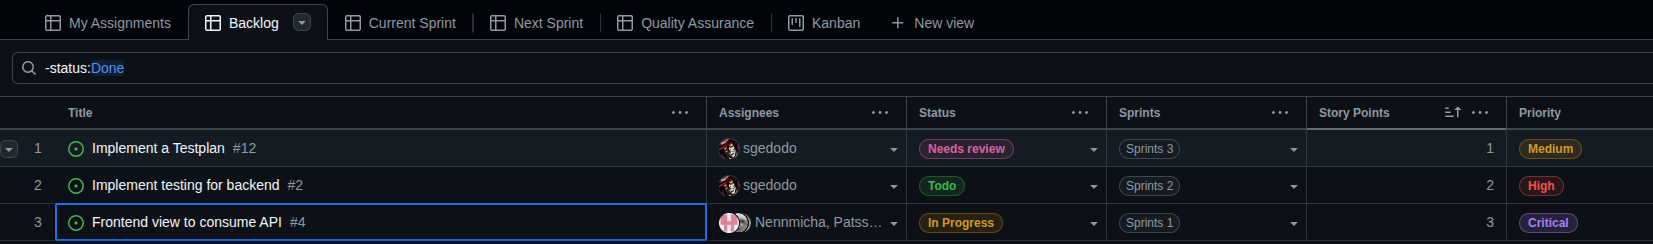
\includegraphics[width=\textwidth]{backlog.png}
  \end{figure}
\end{frame}

\begin{frame}
  \frametitle{Projektmanagement mit Scrum \& GitHub Projects}
  \begin{figure}[h]
    \caption{Screenshot der GitHub Projects Ansicht der Quality Assurance}
    \centering
    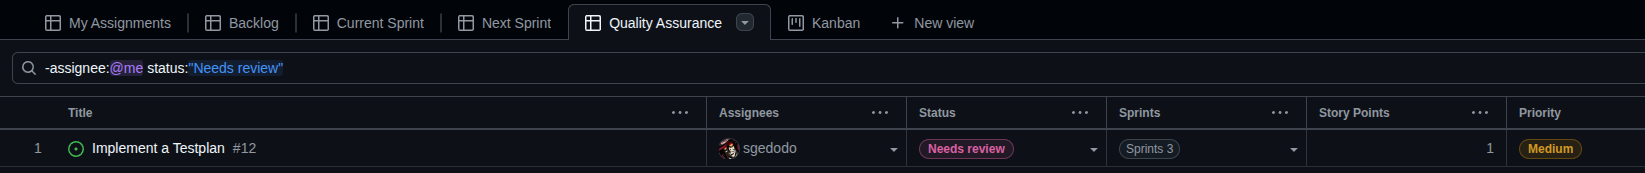
\includegraphics[width=\textwidth]{quality_assurance.png}
  \end{figure}
\end{frame}

\begin{frame}
  \frametitle{Projektmanagement mit Scrum \& GitHub Projects}
  \begin{figure}[h]
    \caption{Screenshot der GitHub Ansicht einer Story}
    \centering
    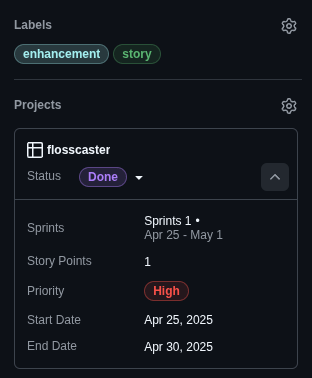
\includegraphics[width=.3\textwidth]{overview.png}
  \end{figure}
\end{frame}

\section{Mockup-Design und Gestaltung \small{(Patryk Brychcy \& Michael Filatoff)}}
\begin{frame}
  \frametitle{Mockup-Design und Gestaltung}
  \begin{figure}[h]
    \caption{Figma Design der Landingpage}
    \centering
    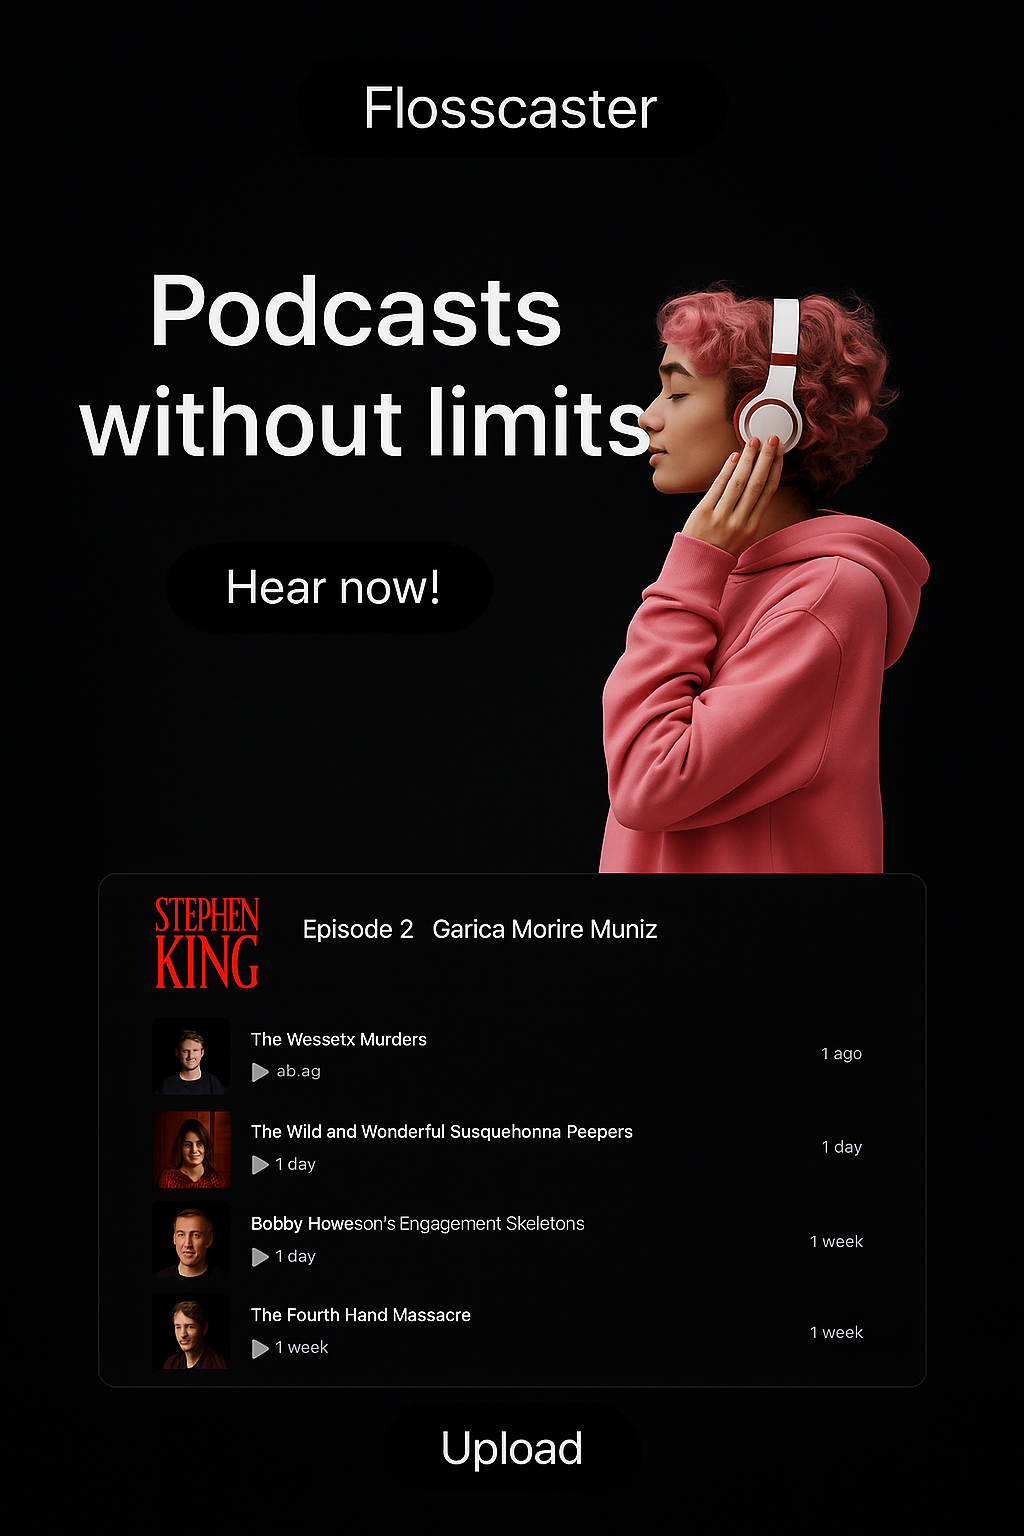
\includegraphics[width=0.4\textwidth]{flosscaster1.png}
  \end{figure}
\end{frame}

\begin{frame}
  \frametitle{Mockup-Design und Gestaltung}
  \begin{figure}[h]
    \caption{Figam Design des Upload-Dialogs}
    \centering
    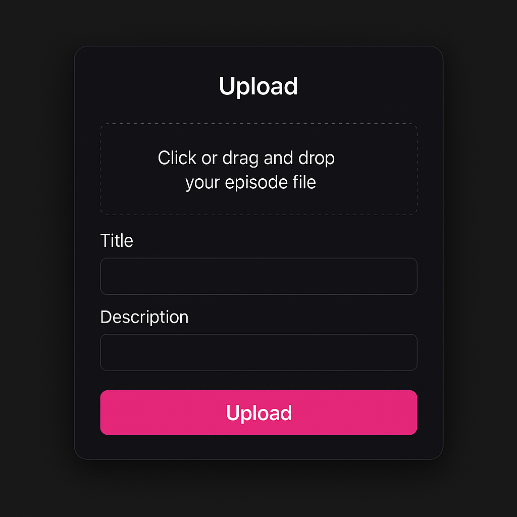
\includegraphics[width=0.3\textwidth]{flosscaster2.png}
  \end{figure}
\end{frame}

\begin{frame}
  \frametitle{Mockup-Design und Gestaltung}
  \begin{figure}[h]
    \caption{Implementiertes Design der Landingpage}
    \centering
    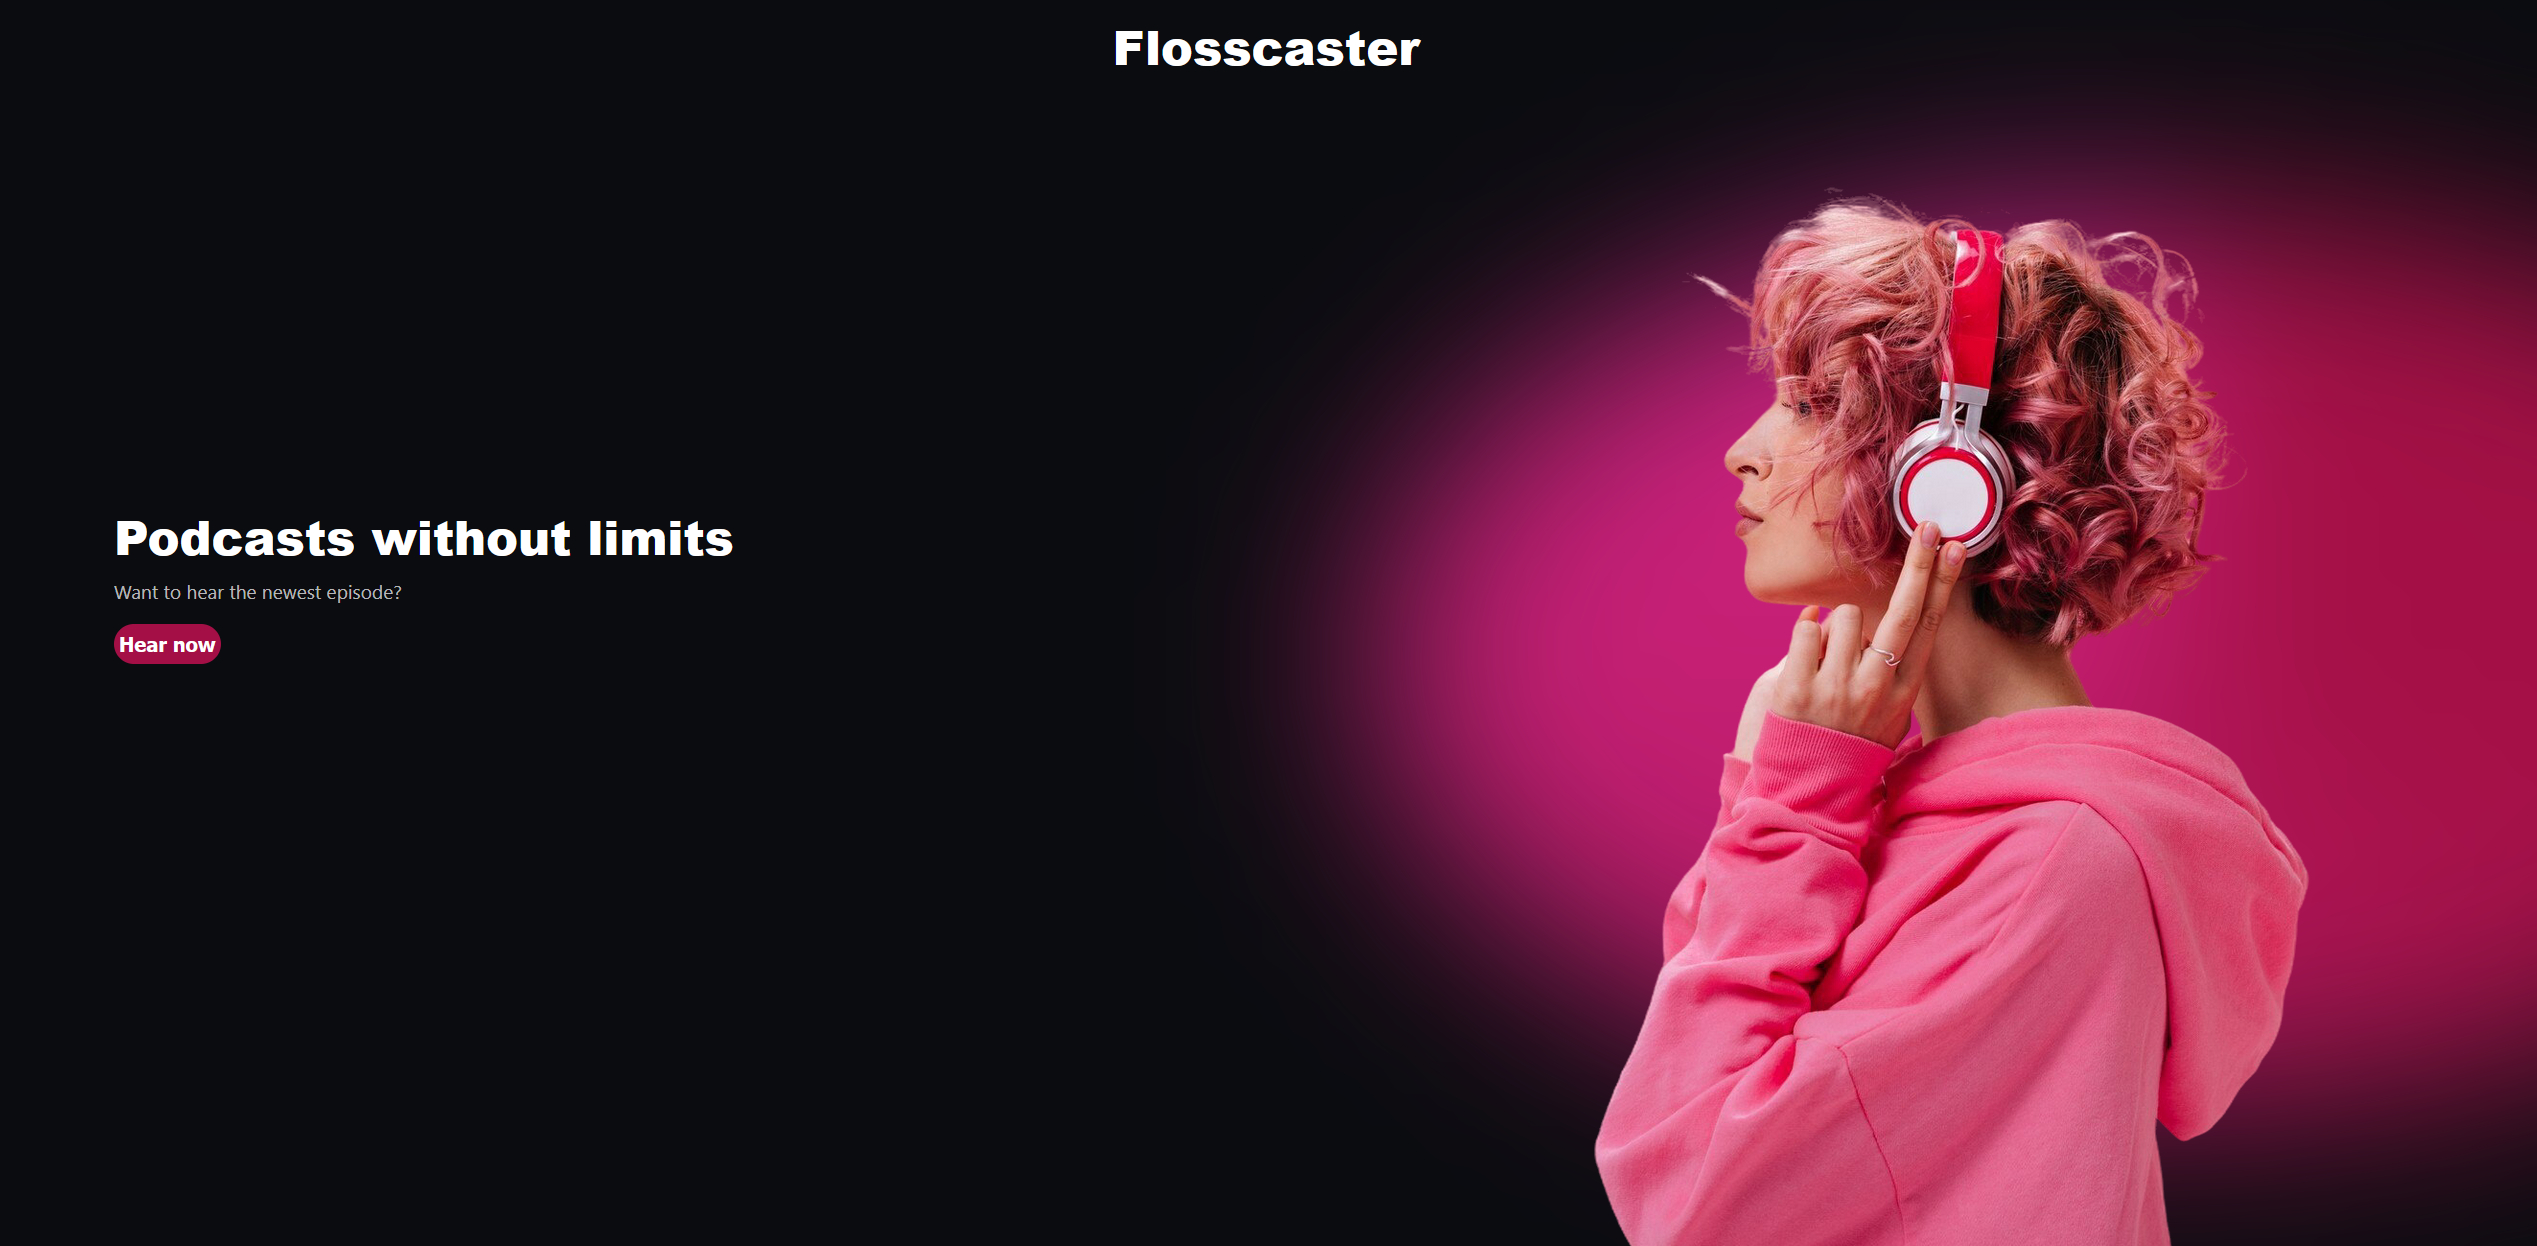
\includegraphics[width=0.7\textwidth]{flosscaster3.png}
  \end{figure}
\end{frame}

\begin{frame}
  \frametitle{Mockup-Design und Gestaltung}
  \begin{figure}[h]
    \caption{Implementiertes Design der Podcast-Episoden}
    \centering
    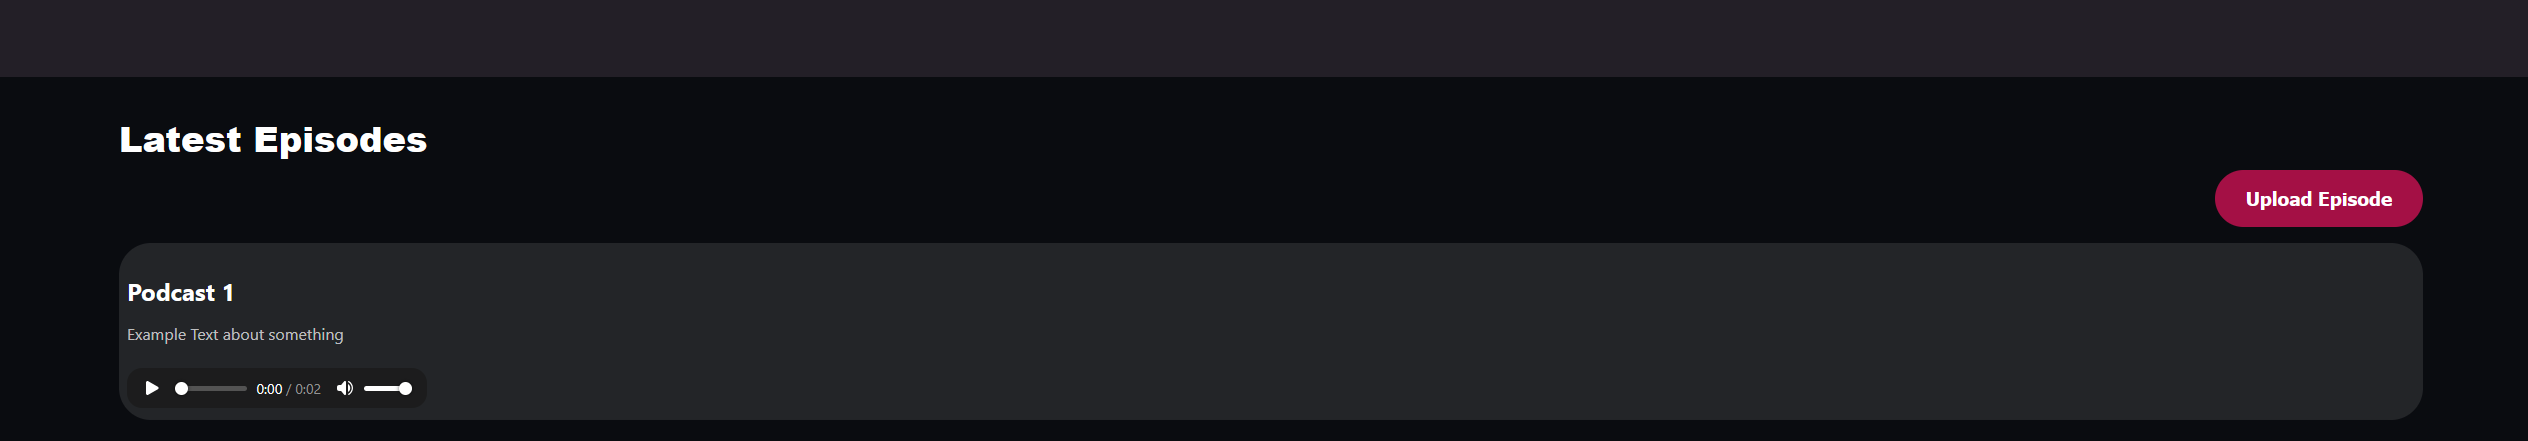
\includegraphics[width=\textwidth]{flosscaster4.png}
  \end{figure}
\end{frame}

\section{Technische Dokumentation}
\subsection{Frontend \small{(Michael Filatoff)}}

\begin{frame}[fragile]
\frametitle{Frontend}
\begin{lstlisting}[label=lst:frontend-hero-image, language=html, caption=Implementation des Hero-Bilds]
<img className={styles.mainPicture} src="./assets/hero\_picture.png" alt="Hero Section"/>
\end{lstlisting}
\end{frame}

\begin{frame}[fragile]
\frametitle{Frontend}
\begin{lstlisting}[label=lst:frontend-navbar, language=html, caption=Implementation der Navbar]
<a href="/" className={styles.mainHeader}>
  Flosscaster
</a>
\end{lstlisting}
\end{frame}

\subsubsection{Styling \small{(Sascha Gav)}}
\begin{frame}
\frametitle{Styling}
\begin{center}
  \huge Styling
\end{center}
\end{frame}

\subsection{Backend \small{(Benedikt Zundel)}}

\begin{frame}[fragile]
\frametitle{Backend}
\begin{lstlisting}[label=lst:episode_model, language=Python, caption=Implementation der Podcast-Episoden Klasse]
@dataclass
class Podcast:
    id: int
    title: str
    description: str
    date: str
    filepath: str
\end{lstlisting}
\end{frame}

\begin{frame}
  \frametitle{Backend}
  \begin{itemize}
    \item \texttt{/api/list}
    \item \texttt{/api/create}
    \item \texttt{/api/get\_upload/<path>}
    \item \texttt{/rss}
  \end{itemize}
\end{frame}

\subsection{Dockerization \small{(Benedikt Zundel)}}
\begin{frame}
\frametitle{Dockerization}
\begin{center}
  \huge Dockerization
\end{center}
\end{frame}

\subsection{Deployment \small{(Benedikt Zundel)}}
\begin{frame}
\frametitle{Deployment}
\begin{center}
  \huge Deployment
\end{center}
\end{frame}

\subsection{RSS-Feed Generator \small{(Alwin Zimmermann)}}

\begin{frame}[fragile]
\frametitle{RSS-Feed Generator}
\begin{lstlisting}[language=Python, caption=Feedparser Bug]
def load_existing_feed(self):
  """Laedt den bestehenden RSS-Feed, falls vorhanden."""
  if os.path.exists(self.feed_file_path):
      feed = feedparser.parse(self.feed_file_path)
      for entry in feed.entries:
          item = {
              'title': entry.title,
              'description': entry.description,
              'date': entry.published if 'published' in entry else datetime.now().isoformat(),
              'enclosure_url': entry.enclosure.href if 'enclosure' in entry else None,
              'enclosure_type': entry.enclosure.type if 'enclosure' in entry else None,
              'enclosure_length': entry.enclosure.length if 'enclosure' in entry else None
          }
          self.items.append(item)
          print(self)
\end{lstlisting}
\end{frame}

\begin{frame}[fragile]
\frametitle{RSS-Feed Generator}
\begin{lstlisting}[language=Python, caption=RSS-Feed Generator imports]
import os
import argparse
import datetime
import pytz
from lxml import etree
\end{lstlisting}
\end{frame}

\begin{frame}[fragile]
\frametitle{RSS-Feed Generator}
\begin{lstlisting}[language=Python, caption=Erstellen eines neuen Feed-Items]
# Erstelle ein neues Item
new_item = etree.Element('item')
etree.SubElement(new_item, 'title').text = title
etree.SubElement(new_item, 'description').text = description
etree.SubElement(new_item, 'pubDate').text = new_episode_pubDate
enclosure = etree.SubElement(new_item, 'enclosure')
enclosure.set('url', url)
enclosure.set('length', length)
enclosure.set('type', 'audio/mpeg')
\end{lstlisting}
\end{frame}

\subsection{Publikation auf einem Social Media Feed \small{(Dwipa Flügel)}}
\begin{frame}[fragile]
\frametitle{Publikation auf einem Social Media Feed}
\begin{lstlisting}[language=Python, caption=Vollständige Funktion des \textit{Autotootings}]
def masttoot(title: str, url: str, description: str):
    """Publishes a new toot using the input, also sends a reply to the announcement with the description."""

    post_text = "The Flosscasters have released a new podcast episode: " + title + ". Check it out @ " + url

    #Mastodon-Instanz
    mastodon = Mastodon(
        client_id = os.getenv("MASTODON_CLIENT_KEY"),
        client_secret = os.getenv("MASTODON_CLIENT_SECRET"),
        access_token = os.getenv("MASTODON_ACCESS_TOKEN"),
        api_base_url = os.getenv("MASTODON_BASE_URL")
    )

    #Publish the toot and reply to it with the description
    to_reply = mastodon.status_post(post_text)
    mastodon.status_post(description, in_reply_to_id=to_reply.id)
\end{lstlisting}
\end{frame}

\section{Testbericht \small{(Dominik Lepore)}}
\begin{frame}[fragile]
\frametitle{Testbericht}
\begin{lstlisting}[language=Python, caption=Beispiel einer Fixture]
@pytest.fixture() 
def init_testing(): 
    app.config.update({'TESTING': True}) 
    if not os.path.exists(DATABASE_FILE): 
        con = sqlite3.connect(DATABASE_FILE) 
        cur = con.cursor() 
        cur.execute("CREATE TABLE IF NOT EXISTS podcasts(id INTEGER PRIMARY KEY, title, description, date, filepath)") 
        con.close() 
    yield app 
    app.config.update({'TESTING': False}) 
\end{lstlisting}
\end{frame}

\begin{frame}[fragile]
\frametitle{Testbericht}
\begin{lstlisting}[language=Python, caption=Test-Implementation von \texttt{/api/create}]
@pytest.mark.parametrize("title, description, audio", [ 
    ("First FLOSScast", "The very first flosscast", generate_mp3_tts("Hello to the very first flosscast episode.", lang="en")), 
    (generate_random_ascii(length=10), generate_random_ascii(length=99), generate_mp3_size(1024)), 
    (generate_random_ascii(length=24, letters=False, numbers =False, punctuation=True), generate_random_ascii(length=240, punctuation=True), generate_mp3_duration(30)) 
]) 
 
 
def test_create_podcasts(client, title, description, audio): 
    response = client.post("/api/create", content_type="multipart/form-data", 
                           data={ 
        "title": title, 
        "description": description, 
        "audio": open(audio, 'rb') 
    }) 
    assert response.status_code == 200 
\end{lstlisting}
\end{frame}

\begin{frame}[fragile]
\frametitle{Testbericht}
\begin{lstlisting}[language=Python, caption=Implementation der \texttt{client}-Fixture]
@pytest.fixture() 
def client(init_testing): 
    with app.test_client() as client: 
        yield client 
\end{lstlisting}
\end{frame}

\begin{frame}[fragile]
\frametitle{Testbericht}
\begin{lstlisting}[language=Python, caption=Test-Implementation von \texttt{/api/list}]
def test_list(database_entry_id, client): 
    response = client.get("/api/list") 
    assert response.status_code == 200 
    assert f"\"id\":{database_entry_id}".encode("utf8") in response.data 
    assert b"\"title\":" in response.data 
    assert b"\"date\":" in response.data 
    assert b"\"description\":" in response.data 
    assert b"\"filepath\":" in response.data 
\end{lstlisting}
\end{frame}

\begin{frame}[fragile]
\frametitle{Testbericht}
\begin{lstlisting}[language=Python, caption=Test-Implementation von \texttt{/api/list} gegen eine leere Datenbank]
def test_list_empty_db(empty_database, client): 
    response = client.get("/api/list") 
    assert response.status_code == 200 
    assert b'[]' in response.data 
\end{lstlisting}
\end{frame}

\begin{frame}[fragile]
\frametitle{Testbericht}
\begin{lstlisting}[language=Python, caption=Test-Implementation von \texttt{/api/get\_upload}]
def test_getFileByFilename(upload_file, client): 
    response = client.get(f"/api/get_upload/{upload_file}") 
    assert response.status_code == 200 

    assert "audio/mpeg" in response.headers["content-type"] 
\end{lstlisting}
\end{frame}

\begin{frame}[fragile]
\frametitle{Testbericht}
\begin{lstlisting}[language=Python, caption=Test-Implementation von \texttt{/rss}]
def test_getrss(create_rss, client): 
    response = client.get("/rss") 
    assert "application/xml" in response.headers["content-type"] 
    assert response.status_code == 200 or response.status_code == 304 
\end{lstlisting}
\end{frame}

\begin{frame}[fragile]
\frametitle{Testbericht}
\begin{lstlisting}[language=Python, caption=Fixture zum löschen des RSS-Feeds]
@pytest.fixture() 
def delete_rss(init_testing): 
    rss_path = os.getenv("RSS_FILE") 
    if os.path.exists(rss_path): 
        file = open(rss_path, "r") 
        rss_file = file.read() 
        file.close() 
        os.remove(rss_path) 
        return rss_file 
    return "failure" 
\end{lstlisting}
\end{frame}

\begin{frame}[fragile]
\frametitle{Testbericht}
\begin{lstlisting}[language=Python, caption=Test-Implementation von \texttt{/rss} bei nicht vorhandenem Feed]
def test_getrss_no_file(delete_rss, client): 
    response = client.get("/rss") 
    assert response.status_code == 404 
    if not delete_rss == "failure": 
        rss_path = os.getenv("RSS_FILE") 
        with open(rss_path, "w") as file: 
            file.write(delete_rss) 
\end{lstlisting}
\end{frame}

\subsection{Static Code-Analyse (Deniz Karaman)}
\begin{frame}
\frametitle{Static Code-Analyse}
\begin{center}
  \huge Static Code-Analyse
\end{center}
\end{frame}

\end{document}
